\documentclass{article}

\usepackage{amsmath}
\usepackage{amssymb}
\usepackage{amsfonts}
\usepackage[margin=1in]{geometry}
\usepackage{titling}
\usepackage{shellesc}
\usepackage{minted}
\usepackage{graphicx}
\usepackage{siunitx}
\usepackage[bookmarks]{hyperref}
\usepackage{xcolor}
\hypersetup{
    colorlinks,
    linkcolor={red},
    citecolor={blue!50!black},
    urlcolor={blue!80!black}
}

\setlength{\droptitle}{-7em}

\title{Supporting Calculations}
\author{Group 701: Ivy Tan, Tyler Tian, Julia Ye (TA: Laurence Yin)}

\begin{document}

\maketitle
\sloppy

\section{Source Code}

The code is split into two parts: A Python module that does all the calculations (\ref{sec:calc}), and another module
that provides a command-line interface (CLI) (\ref{sec:cli}).

Bridge designs are given to the program in YAML files. The specification for Design 0 (\ref{sec:design0}) and the final
design (\ref{sec:design}) are listed here.

The code depends on the following packages:
\begin{itemize}
    \setlength\itemsep{0em}
    \item \texttt{numpy}
    \item \texttt{matplotlib}
    \item \texttt{pyyaml}
    \item \texttt{click} (CLI only)
\end{itemize}

\subsection{Calculations Code (\texttt{calculate.py})}
\label{sec:calc}

Sample usage of the functions to do the calculations is included at the end of this code listing. All functions are
documented with docstrings, which includes example calls.

\inputminted[linenos, breaklines, fontsize=\small]{python}{../../calculate.py}
\pagebreak

\subsection{Command-Line Interface Code (\texttt{bridgedesigner.py})}
\label{sec:cli}

\inputminted[linenos, breaklines, fontsize=\small]{python}{../../bridgedesigner.py}
\pagebreak

\subsection{Bridge Specification Code}

\subsubsection{Design 0 (\texttt{design0.yaml})}
\label{sec:design0}

\inputminted[linenos, breaklines, fontsize=\small]{yaml}{../../design0.yaml}
\pagebreak

\subsubsection{Final Design (\texttt{bridge.yaml})}
\label{sec:design}

\inputminted[linenos, breaklines, fontsize=\small]{yaml}{../../new.yaml}
\pagebreak

\section{Handwritten Calculations}

Manual calculations are shown below for verification of the code. All calculations are for Design 0.

\subsection{Internal Forces}

Verifies reaction forces, shear force diagrams, and bending moment diagrams as computed by
\mintinline{python}{Bridge.reaction_forces()}, \mintinline{python}{Bridge.make_sfd()}, and
\mintinline{python}{Bridge.make_bmd()}. These numbers can be obtained by running
\texttt{python3 bridgedesigner.py design0.yaml load point 200} and
\texttt{python3 bridgedesigner.py design0.yaml load train 280}, or
\begin{minted}[linenos, breaklines, fontsize=\small]{python}
    with open("design0.yaml", "r", encoding="utf-8") as f:
        bridge = Bridge.from_yaml(f)
    
    forces = bridge.load_points(200)
    forces = bridge.reaction_forces(forces)
    # SFD for point load P = 200
    sfd_point = bridge.make_sfd(forces)
    # BMD for point load P = 200
    bmd_point = bridge.make_bmd(sfd)

    forces = bridge.load_train(280)
    forces = bridge.reaction_forces(forces)
    # SFD for train load
    sfd_train = bridge.make_sfd(forces)
    # BMD for train load
    bmd_train = bridge.make_bmd(sfd)
\end{minted}

\begin{figure}[H]
    \centering
    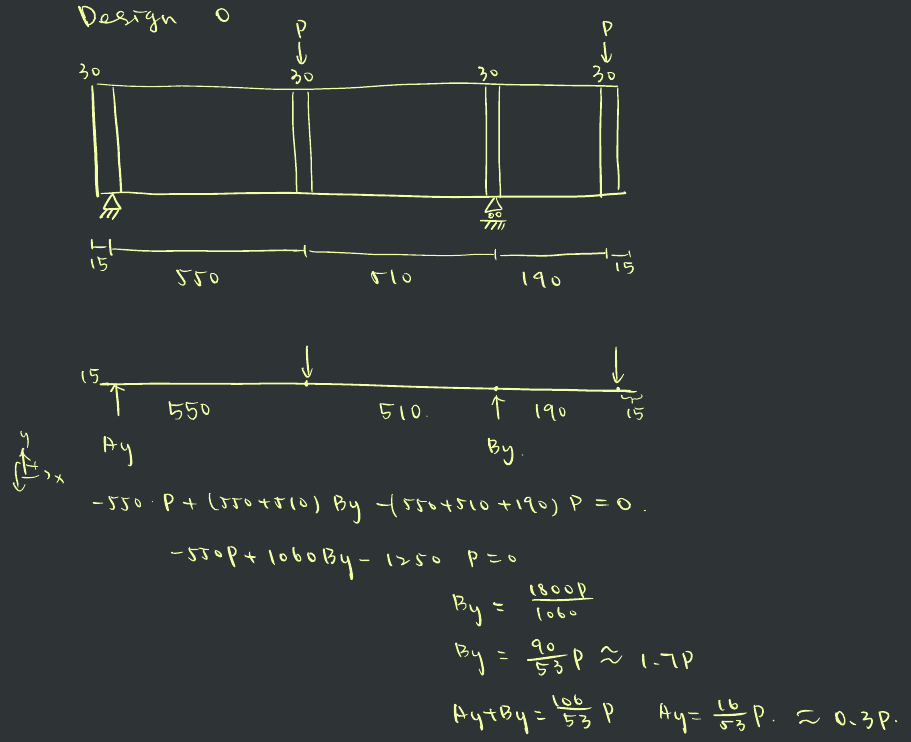
\includegraphics[width=0.49\textwidth]{forces.png}
    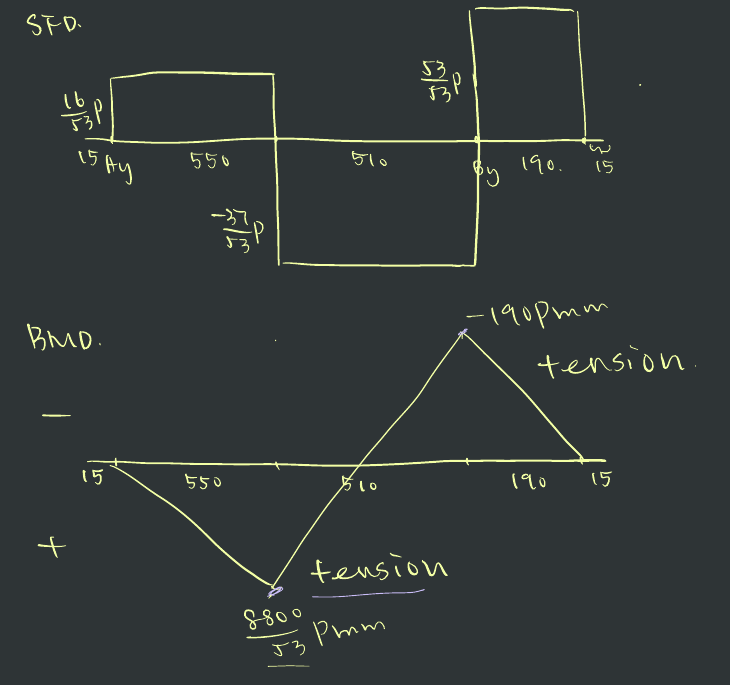
\includegraphics[width=0.49\textwidth]{sfd_bmd.png}
    \caption{Reaction forces, SFD and BMD (point loading).}
\end{figure}

\begin{figure}[H]
    \centering
    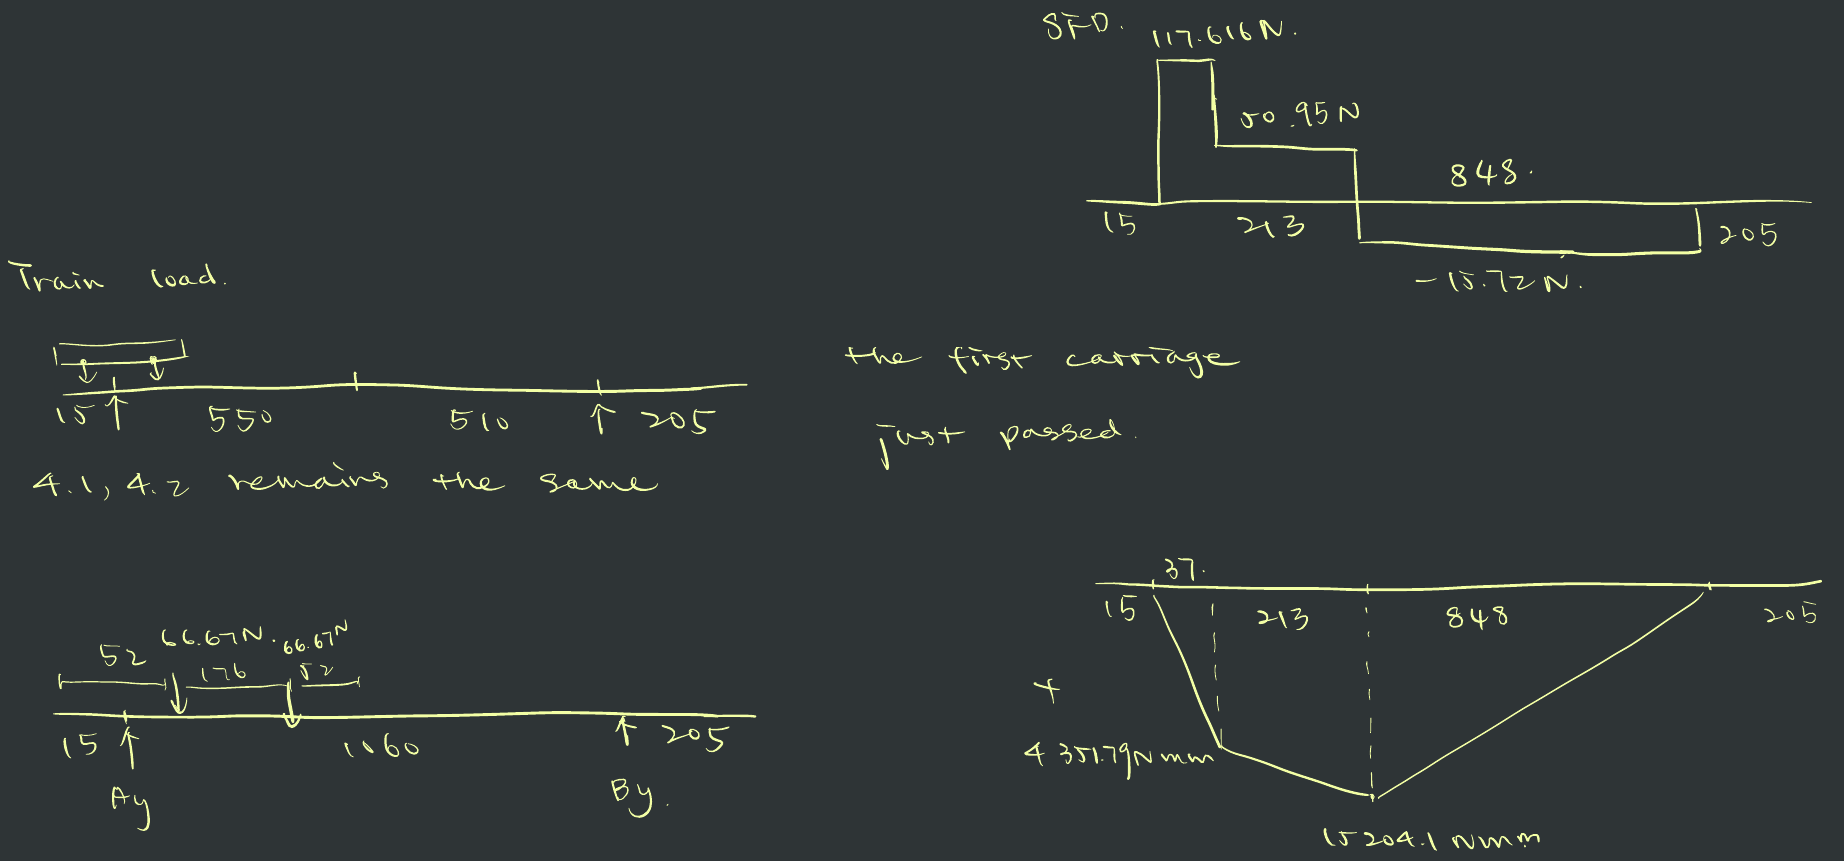
\includegraphics[width=\textwidth]{train.png}
    \caption{Reaction forces, SFD and BMD (one case of train loading).}
\end{figure}

\subsection{Cross-Sectional Properties}

Verifies cross-sectional properties computed by the \mintinline{python}{CrossSection} class.
These numbers can be obtained by running \texttt{python3 bridgedesigner.py design0.yaml geometry}, or
\begin{minted}[linenos, breaklines, fontsize=\small]{python}
    with open("design0.yaml", "r", encoding="utf-8") as f:
        bridge = Bridge.from_yaml(f)
    cs = bridge.cross_sections[0][2]
    print("Area:", cs.area)
    print("Centroid:", cs.ybar)
    print("I:", cs.i)
    print("Centroidal Q:", cs.calculate_q(cs.ybar))
\end{minted}

\begin{figure}[H]
    \centering
    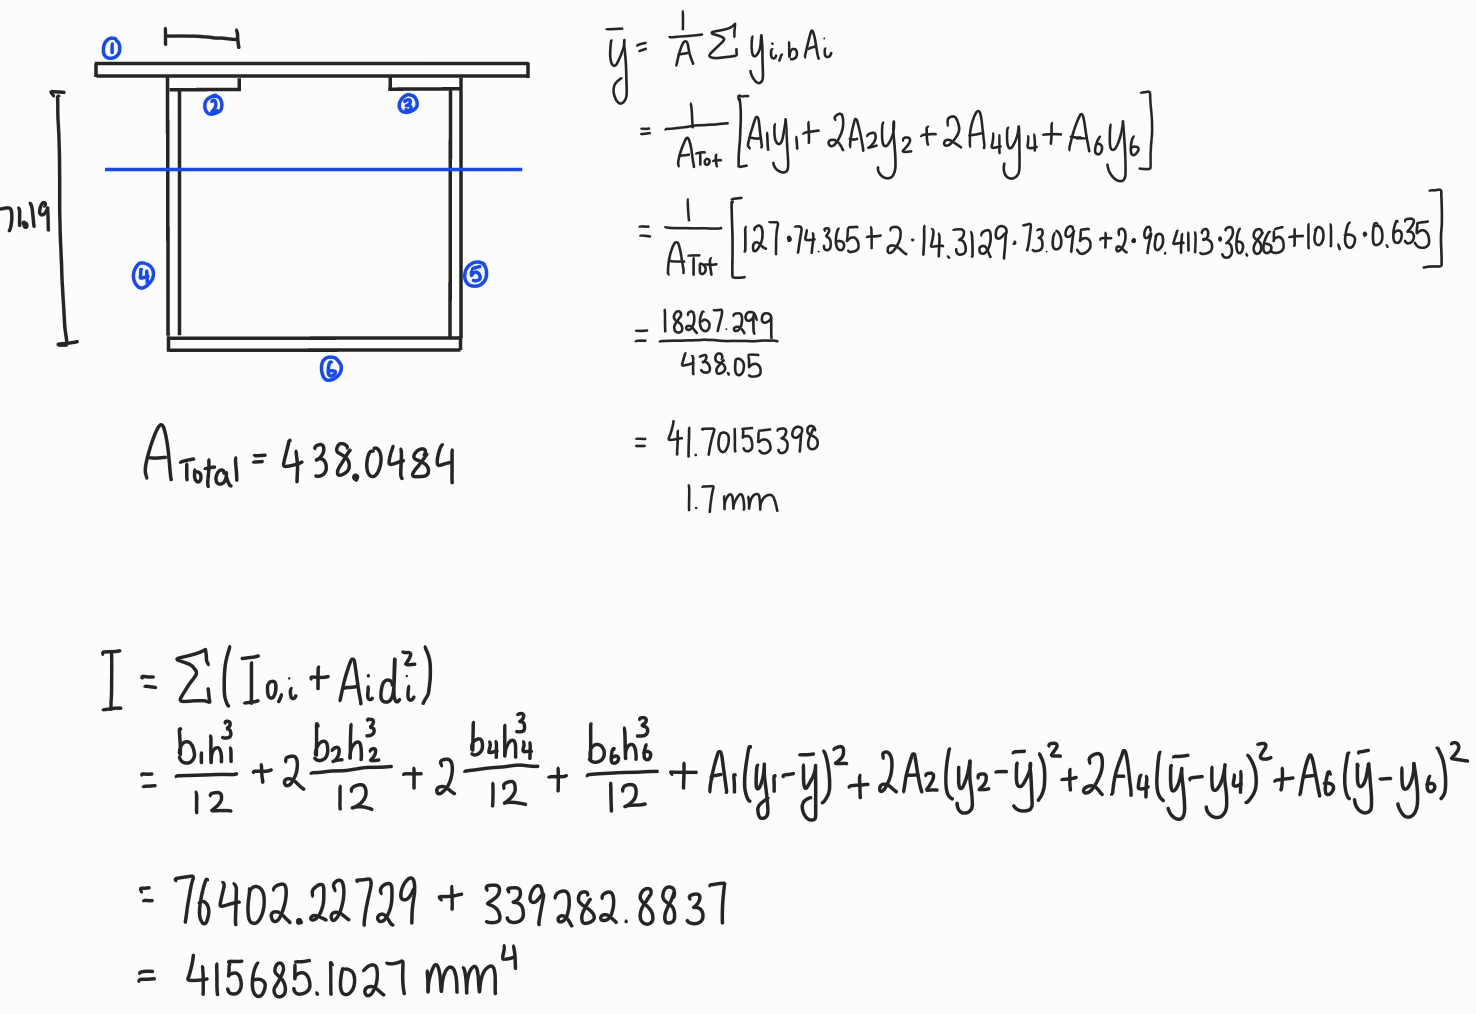
\includegraphics[width=0.75\textwidth]{crosssection.png}
    \caption{Cross-sectional geometry.}
\end{figure}

\begin{figure}[H]
    \centering
    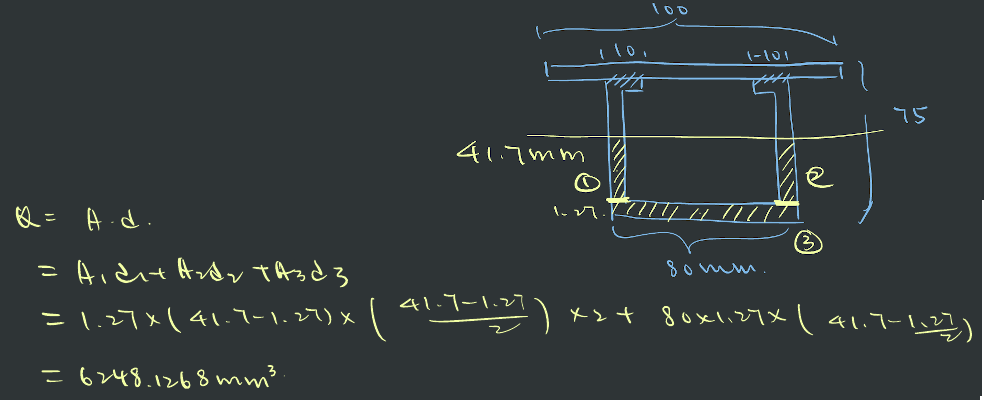
\includegraphics[width=0.7\textwidth]{qcent.png}
    \caption{Computing \(Q\) at the centroidal axis.}
\end{figure}

\subsection{Bridge Capacity}

Verifies various \(M_{fail}\) and \(V_{fail}\) values as computed by the \mintinline{python}{Bridge.calculate_<mode>_mfail()}
and \mintinline{python}{Bridge.calculate_<mode>_vfail()} methods. These numbers can be obtained by running
\texttt{python3 bridgedesigner.py design0.yaml load point 200 --mfail all --vfail all}, or
\begin{minted}[linenos, breaklines, fontsize=\small]{python}
    with open("design0.yaml", "r", encoding="utf-8") as f:
        bridge = Bridge.from_yaml(f)
    
        matboard_vfail = bridge.calculate_matboard_vfail()
    
    matboard_vfail = bridge.calculate_matboard_vfail()
    glue_vfail = bridge.calculate_glue_vfail()
    buckling_vfail = bridge.calculate_buckling_vfail()
    tensile_mfail_upper, tensile_mfail_lower = bridge.calculate_tensile_mfail()
    compressive_mfail_upper, compressive_mfail_lower = bridge.calculate_compressive_mfail()
    one_edge_mfail_upper, one_edge_mfail_lower = bridge.calculate_one_edge_mfail()
    two_edge_mfail_upper, two_edge_mfail_lower = bridge.calculate_two_edge_mfail()
    linear_stress_mfail_upper, linear_stress_mfail_lower = bridge.calculate_linear_stress_mfail()

    vfail = [matboard_vfail, glue_vfail, buckling_vfail]
    mfail_upper = [tensile_mfail_upper,
                   compressive_mfail_upper,
                   one_edge_mfail_upper,
                   two_edge_mfail_upper,
                   linear_stress_mfail_upper]
    mfail_lower = [tensile_mfail_lower,
                   compressive_mfail_lower,
                   one_edge_mfail_lower,
                   two_edge_mfail_lower,
                   linear_stress_mfail_lower]
    # Factor of safety against shear
    fos_shear = bridge.calculate_shear_fos(sfd, vfail)
    # Factor of safety against bending moment
    fos_moment = bridge.calculate_moment_fos(bmd, mfail_upper, mfail_lower)
\end{minted}

\subsubsection{Shear Failure}

\begin{figure}[H]
    \centering
    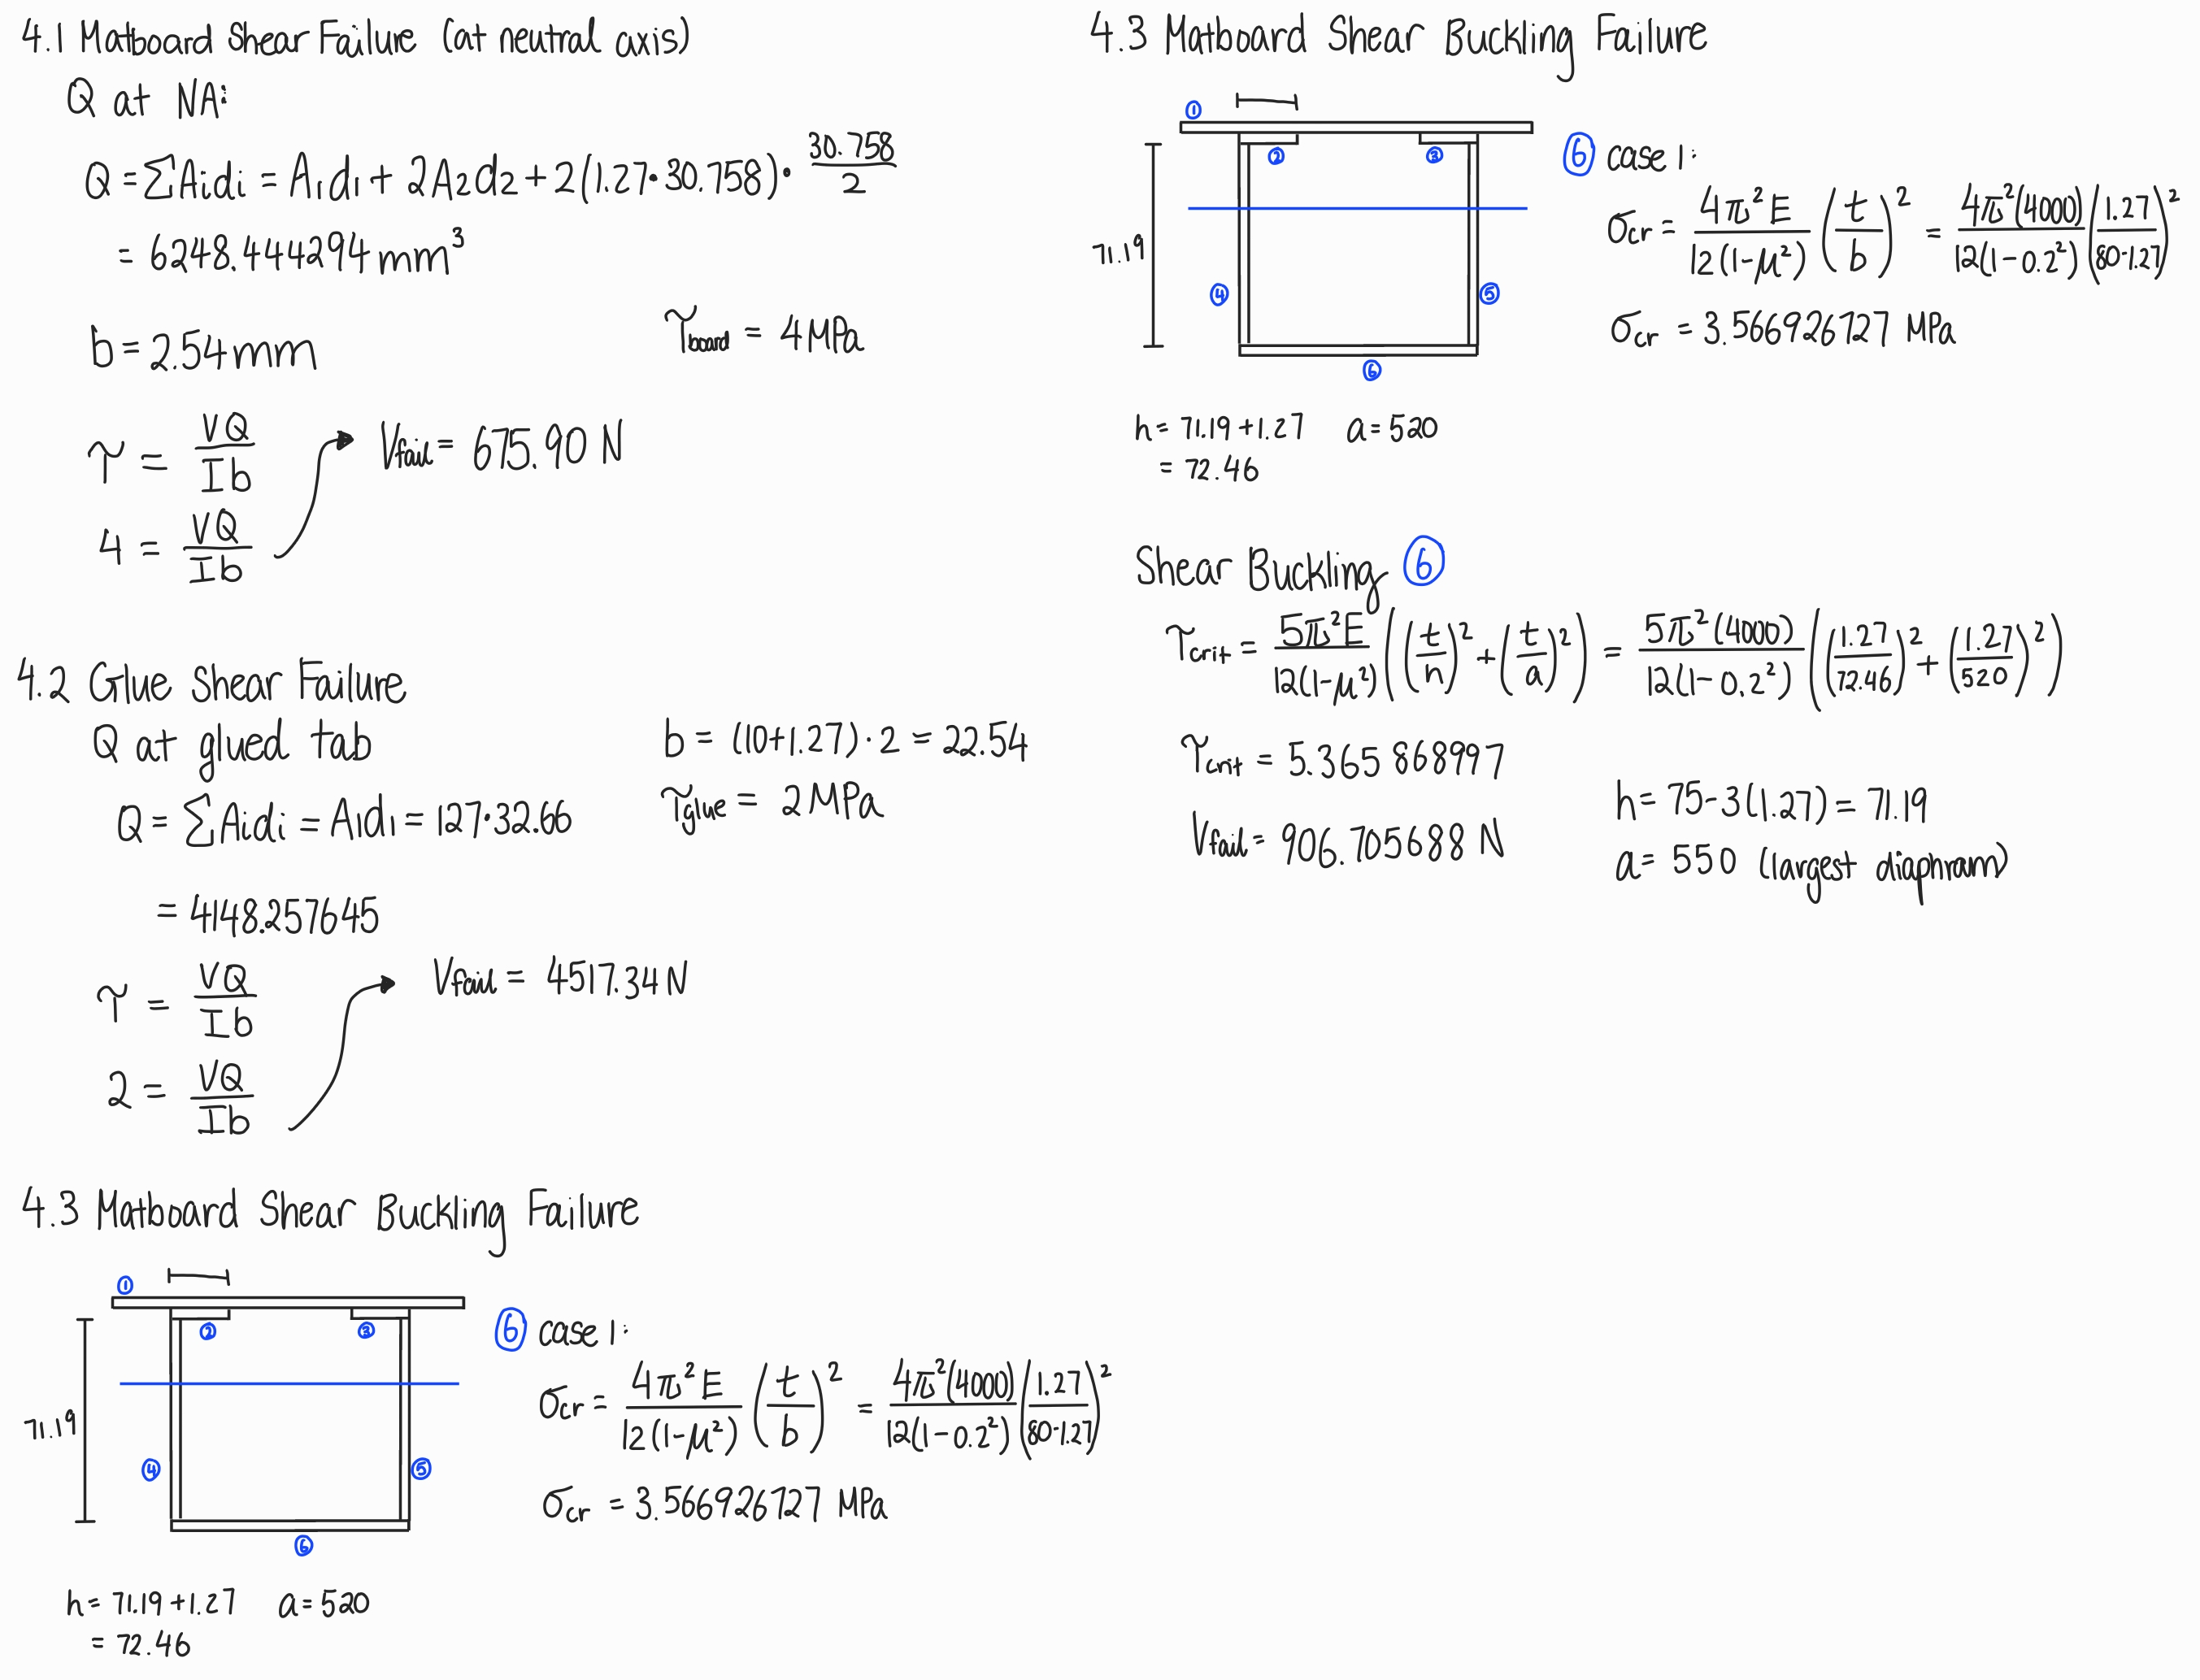
\includegraphics[width=\textwidth]{shear.png}
    \caption{Failure shear force calculations.}
\end{figure}

\subsubsection{Bending Moment Failure}

Note two values are calculated for each one because the values could be different depending on whether the top or the
bottom is in compression/tension.

\begin{figure}[H]
    \centering
    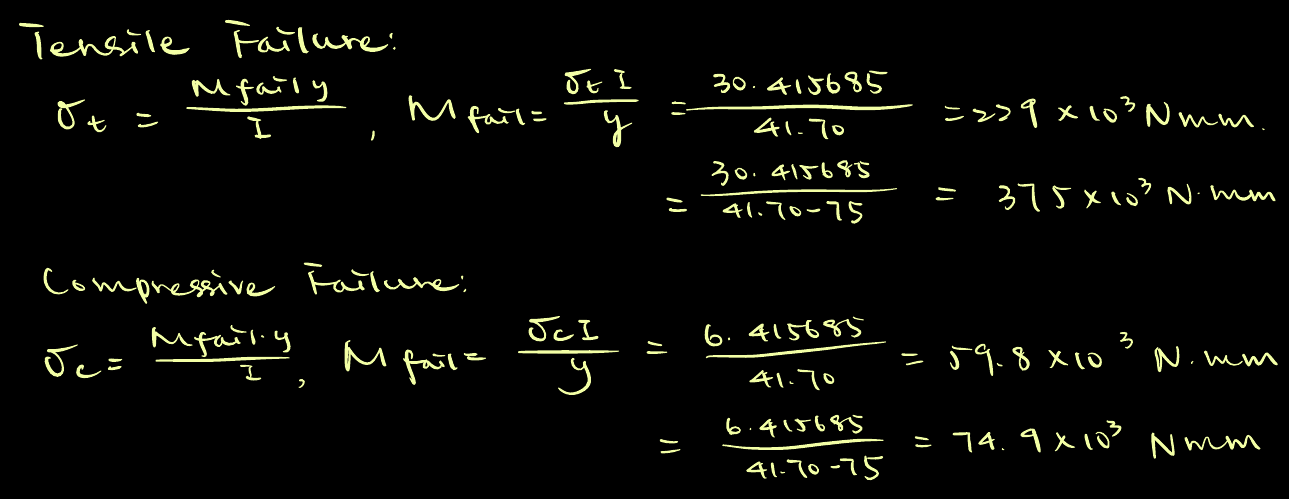
\includegraphics[width=\textwidth]{tensile_compressive_failure.png}
    \caption{Tensile and compressive \(M_{fail}\) calculation.}
\end{figure}

\begin{figure}[H]
    \centering
    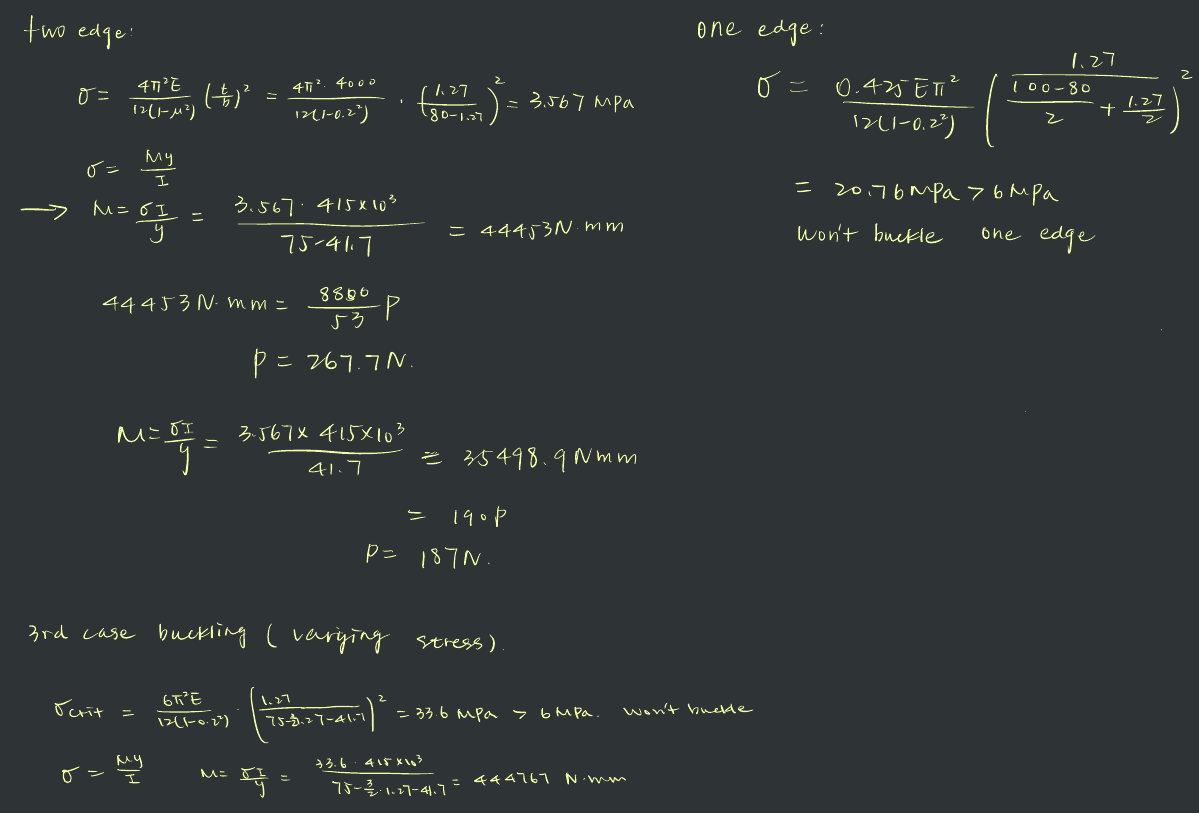
\includegraphics[width=\textwidth]{localbuckling.png}
    \caption{3 cases of local buckling.}
    \label{fig:local_buckling}
\end{figure}

\subsubsection{Factors of Safety}

Verifies \mintinline{python}{Bridge.calculate_shear_fos()} and \mintinline{python}{Bridge.calculate_moment_fos()}.

Failure shear force was determined previously to be \(675.90\si{N}\) (from matboard shear). Therefore
\(\text{FoS}_{\text{shear}} = \frac{675.90}{238} = 2.84\).

Failure bending moment was determined previous to be
\(\SI{44.5e3}{N.mm}\) (from local buckling of the middle top flange, with two edges restrained). Therefore
\(\text{FoS}_{\text{moment}} = \frac{\num{44.5e3}}{\num{55.5e3}} = 0.802\) (i.e. the bridge fails by bending).

Note the maximum shear force and bending moment demand used here are determined by
\mintinline{python}{Bridge.max_sfd_train()} and \mintinline{python}{Bridge.max_bmd_train()} by sampling over 500 train
positions.

\subsubsection{Failure Load Calculation}

See Figure \ref{fig:local_buckling}. The limiting factor, as described above, is the two-edge local buckling of the middle top
flange. Using this failure moment the failure load is determined to be \(187.1\si{N}\).

\subsection{Midspan Deflection}

\begin{figure}[H]
    \centering
    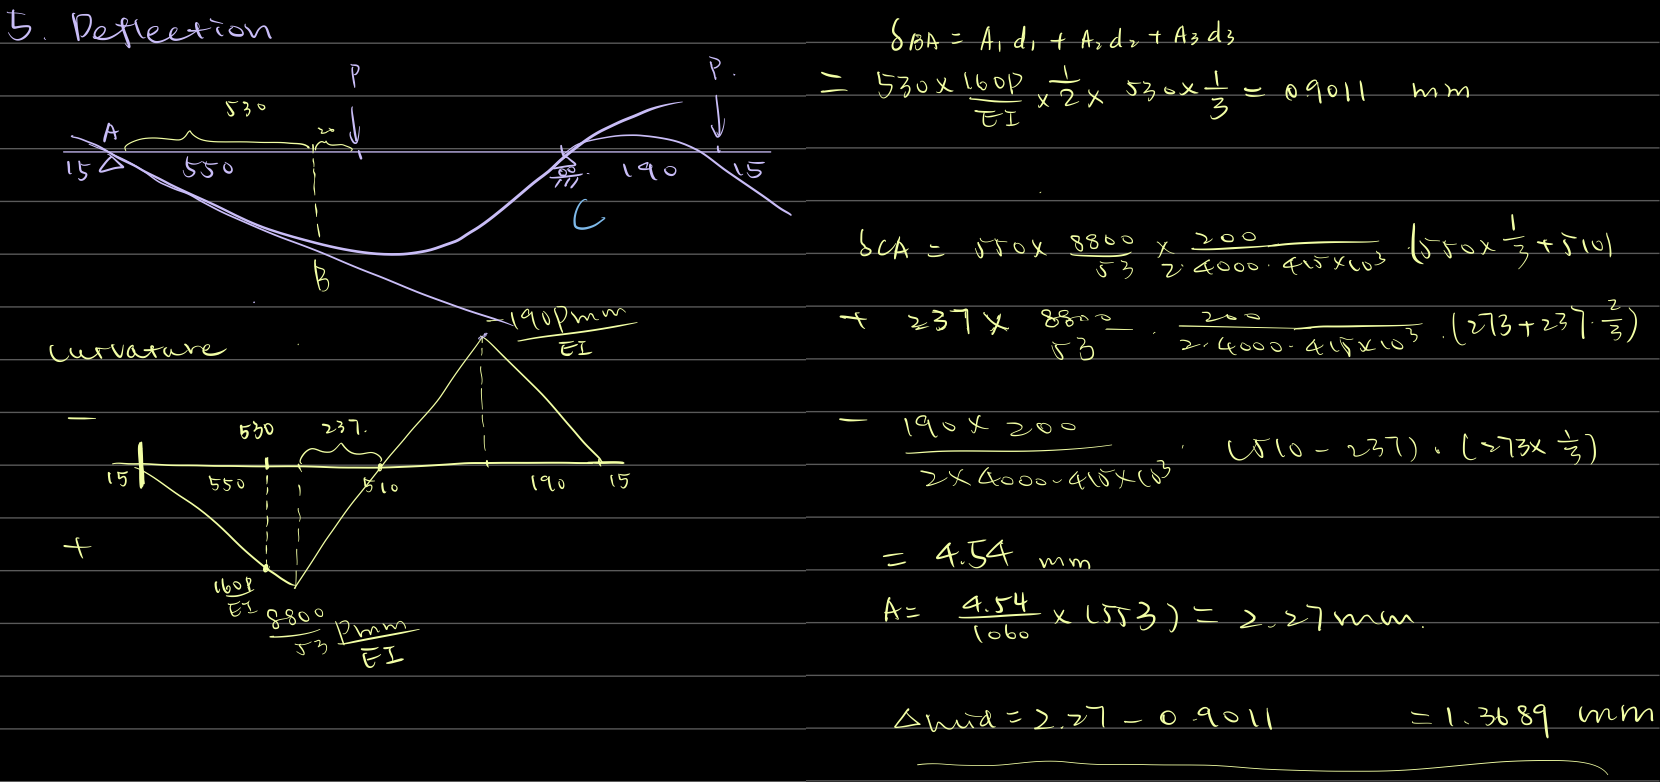
\includegraphics[width=\textwidth]{deflection.png}
    \caption{Midspan deflection calculation.}
\end{figure}

\end{document}
